\documentclass{article}
\usepackage{iclr2026_conference,times}
\input{math_commands.tex}

\usepackage{amsmath}
\usepackage{amssymb}
\usepackage{booktabs}
\usepackage{float}
\usepackage{graphicx}
\usepackage{xcolor}
\usepackage{hyperref}
\hypersetup{colorlinks=true,citecolor=green!45!black,linkcolor=blue!55!black,urlcolor=blue!55!black}
\usepackage{url}

\title{Audit-Then-Sample:\\
Certifying When Diffusion Policies Should Search More Trajectories}

% Leave \iclrfinalcopy commented for anonymous review submissions.
\author{Anonymous Authors\\Paper under double-blind review}

\newcommand{\ats}{Audit-Then-Sample}
\newcommand{\maxsel}{maximum-score selection}
\newcommand{\ci}{95\% CI}
\newcommand{\lcb}{LCB}
% Generated by experiments/deployment_stress.py; do not edit by hand.
\newcommand{\AtsDeployStressRows}{180}
\newcommand{\AtsDeployStressRegimes}{9}
\newcommand{\AtsDeployStressHarmfulRows}{92}
\newcommand{\AtsDeployStressAdaptiveFalseAdmit}{0.000}
\newcommand{\AtsDeployStressStaticFalseAdmit}{0.000}
\newcommand{\AtsDeployStressFixedHighHarmRate}{0.511}
\newcommand{\AtsDeployStressAuditRate}{1.000}
\newcommand{\AtsDeployStressMeanCheckedN}{16.000}
\newcommand{\AtsDeployStressStaticVsHigh}{0.088}
\newcommand{\AtsDeployStressStaticVsHighCILow}{0.005}
\newcommand{\AtsDeployStressStaticVsHighHarm}{0.450}
\newcommand{\AtsDeployStressStaticVsHighHarmCILow}{0.318}
\newcommand{\AtsDeployStressStaticVsHighNegative}{0.263}
\newcommand{\AtsDeployStressStaticVsHighNegativeCILow}{0.166}
\newcommand{\AtsDeployStressStaticAlignedCost}{-0.316}
\newcommand{\AtsDeployStressStaticAlignedCostCIHigh}{-0.294}
\newcommand{\AtsDeployStressAdaptiveVsHigh}{-0.046}
\newcommand{\AtsDeployStressAdaptiveVsHighCILow}{-0.150}
\newcommand{\AtsDeployStressAdaptiveVsHighHarm}{0.434}
\newcommand{\AtsDeployStressAdaptiveVsHighHarmCILow}{0.297}
\newcommand{\AtsDeployStressFixedHighVsLowHarm}{-0.435}
\newcommand{\AtsDeployStressFixedHighVsLowHarmCIHigh}{-0.324}

% Auto-generated by experiments/fetch_robotics_benchmark.py
\newcommand{\AtsFetchBenchmarkEnv}{FetchPush-v4}
\newcommand{\AtsFetchBenchmarkUnits}{12}
\newcommand{\AtsFetchBenchmarkCandidateRollouts}{1152}
\newcommand{\AtsFetchBenchmarkCurveRows}{4608}
\newcommand{\AtsFetchBenchmarkAlignedGain}{0.007}
\newcommand{\AtsFetchBenchmarkAlignedCILow}{0.006}
\newcommand{\AtsFetchBenchmarkMisalignedChange}{0.001}
\newcommand{\AtsFetchBenchmarkMisalignedCIHigh}{0.012}
\newcommand{\AtsFetchBenchmarkAntiOracleChange}{-0.031}
\newcommand{\AtsFetchBenchmarkAntiOracleCIHigh}{-0.016}
\newcommand{\AtsFetchBenchmarkOracleGap}{0.057}
\newcommand{\AtsFetchBenchmarkSuccessGain}{0.000}
\newcommand{\AtsFetchBenchmarkProgressGain}{0.000}
\newcommand{\AtsFetchBenchmarkRuntimeMin}{117.33}
\newcommand{\AtsFetchBenchmarkRuntimeMax}{775.28}


\begin{document}
\maketitle

\begin{abstract}
Diffusion action policies can sample many candidate trajectories for a single observation, making test-time trajectory search an attractive but risky knob. This paper asks when the extra sampling is actually useful. We study finite observation-conditioned candidate pools in which each trajectory has a selection score and a measured task utility. A tie-aware selection law shows that larger $N$ always improves selected score, but need not improve real utility: the outcome depends on candidate diversity, upper-tail score--utility alignment, and latency. We propose \ats{}, an inference-time controller that admits high-$N$ sampling only when empirical lower-bound gates certify diversity, tail utility, utility gain, and latency-adjusted gain; otherwise it abstains, audits rollouts, repairs the scorer, increases diversity, reduces denoising depth, stops early, or blocks high-$N$ selection. The evidence is CPU-simulation evidence: controlled action samplers, learned state and small-image diffusion-policy-lite denoisers, true epsilon-prediction DDPM/DDIM action diffusion, PushT and FetchPush simulator rollouts, and a \AtsDeployStressRows-row sequential deployment stress suite. The audited full run supports the conditional claim and rejects universal high-$N$ improvement: true DDPM, PushT, and FetchPush aligned oracle reranking improve under high $N$, while anti-correlated or anti-oracle scorers are harmful and the controller has zero false admits in harmful negative controls.
\end{abstract}

\section{Introduction}

Diffusion Policy-style controllers generate action trajectories by iterative denoising conditioned on the current observation \citep{chi2023diffusionpolicy,ho2020ddpm,song2020ddim}. Because generation is stochastic, a deployment can sample multiple trajectories, score them with a critic, value model, likelihood proxy, or reranker, and execute the highest-scoring candidate. This creates a simple practical question: how many diffusion trajectories should a robot sample?

The naive answer is ``more''. If the score is aligned with real task utility, more candidates increase the chance of finding a good trajectory. Yet the same maximization can amplify artifacts. A scorer that rewards shortcuts, risky modes, duplicated samples, or likelihood quirks can become worse as $N$ increases because maximum-score selection searches harder through the scorer's upper tail. This failure is not visible from selected score alone, and it can survive moderate average score--utility correlation. What matters is the finite joint distribution of score and utility in the high-score tail.

We study maximum-score trajectory selection over sampled action trajectories. For a fixed observation $o$, a generator produces a finite pool $\{(\tau_i,S_i,U_i)\}_{i=1}^M$, where $\tau_i$ is an action trajectory, $S_i$ is the selection score, and $U_i$ is measured task utility after optional latency cost. The selector draws $N$ candidates and executes the one with maximum score. This framing separates three mechanisms: diversity determines whether additional candidates expose new options; upper-tail alignment determines whether high-score candidates are high-utility candidates; and latency determines whether extra sampling remains worthwhile.

Our contribution is a diagnose-predict-control framework, not a broad robot benchmark suite.

\begin{enumerate}
\item We give a finite, tie-aware trajectory-selection law that separates monotone selected-score improvement from real-utility improvement.
\item We introduce \ats{}, a conservative controller that certifies high-$N$ only under lower-bound evidence and otherwise emits an abstention or repair action.
\item We test the mechanism across controlled samplers, learned diffusion-policy-lite models, true action DDPM/DDIM sampling, PushT and FetchPush simulator rollouts, and sequential deployment stress.
\item We package each headline claim with CSV/JSON provenance, confidence intervals, negative controls, and overclaim checks.
\end{enumerate}

\section{Finite Selection Law}

For one observation, sort the finite pool by nondecreasing score. Let a score-tie group $g$ occupy ranks $a_g,\ldots,b_g$ among $M$ candidates and let $\bar U_g$ be the mean utility in that tied group. Sampling with replacement and breaking top-score ties uniformly, the expected selected utility is
\begin{equation}
\mathbb{E}[U_{N}^{\mathrm{sel}}]
= \sum_g \bar U_g
\left[
\left(\frac{b_g}{M}\right)^N
- \left(\frac{a_g-1}{M}\right)^N
\right].
\label{eq:finite-law}
\end{equation}
The same expression with $\bar S_g$ gives selected score. Equation~\ref{eq:finite-law} immediately gives selected-score monotonicity in $N$, because the maximum score over a larger sample cannot decrease in expectation. It does not give selected-utility monotonicity. Utility improves only when mass that enters the high-score tail also has high real utility; utility saturates when the pool is collapsed; and utility can decrease when the score tail is anti-aligned with the task.

The controller uses this law as an audited finite-population object. Candidate diversity is summarized by effective sample diversity, pairwise trajectory distance, duplicate collapse rate, cluster count, and cluster entropy. Tail alignment is summarized by score--utility correlation, upper-tail rank correlation, top-score-tail utility, high-$N$ regret, and oracle-minus-scorer gaps. Runtime is represented by measured or modeled cost $C(N,K)$ for sample count $N$ and denoising depth $K$, with latency-adjusted utility $U-\lambda C(N,K)$.

\section{\ats{}}

\ats{} converts the diagnostics into an inference-time decision. Its inputs are candidate trajectories and scores, optional audited utilities from pilot rollouts, a candidate $N,K$ grid, diversity diagnostics, a runtime model or measured runtimes, and risk budget $\delta$. Its output is a selected $N,K$, a decision label, confidence diagnostics, and one recommendation from \{\texttt{increase\_N}, \texttt{stop\_early}, \texttt{reduce\_K}, \texttt{calibrate\_scorer}, \texttt{audit\_rollouts}, \texttt{increase\_diversity}, \texttt{block\_high\_N}\}.

The admission rule is deliberately one-sided. The controller admits \texttt{increase\_N} only if candidate diversity is sufficient; empirical-Bernstein lower bounds \citep{maurer2009empirical} on high-minus-low utility gain, top-score-tail utility, and latency-adjusted gain are positive; and high-score-tail harm is not plausible under the corresponding upper confidence gate. If utilities are missing, it requests rollout auditing or calibration. If the pool is collapsed, it recommends diversity repair. If the upper tail is anti-aligned or high-$N$ utility is harmful, it blocks high-$N$. Isotonic or affine calibration \citep{zadrozny2002transforming,guo2017calibration} is used only when held-out lower-bound gates pass.

Under the bounded audit assumptions used by these confidence gates, if the controller spends total risk $\delta$ across the one-sided tests, then with probability at least $1-\delta$ every admitted \texttt{increase\_N} row has positive audited latency-adjusted high-minus-low gain under the finite audited distribution. This is not a universal improvement theorem: without measured utilities or a valid bound tying scores to real utility, \ats{} abstains.

\begin{figure}[t]
\centering
\begin{minipage}{0.49\linewidth}
\centering
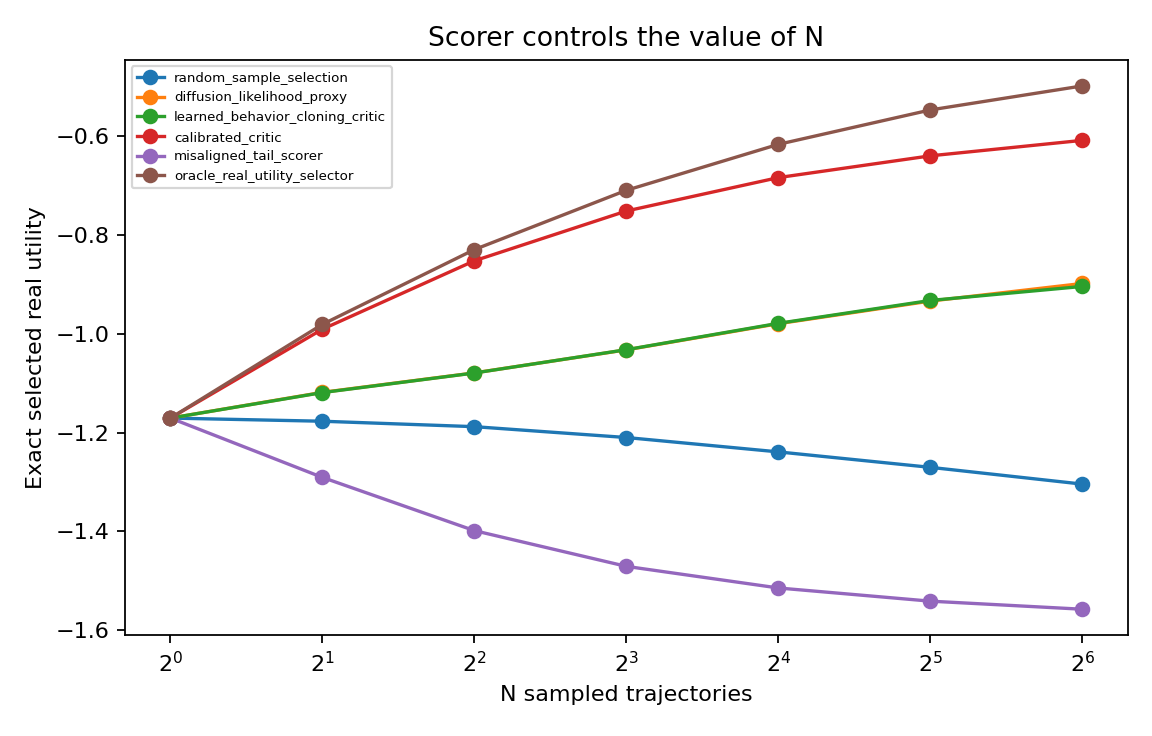
\includegraphics[width=\linewidth]{figures/scorer_comparison.png}
\end{minipage}
\hfill
\begin{minipage}{0.49\linewidth}
\centering
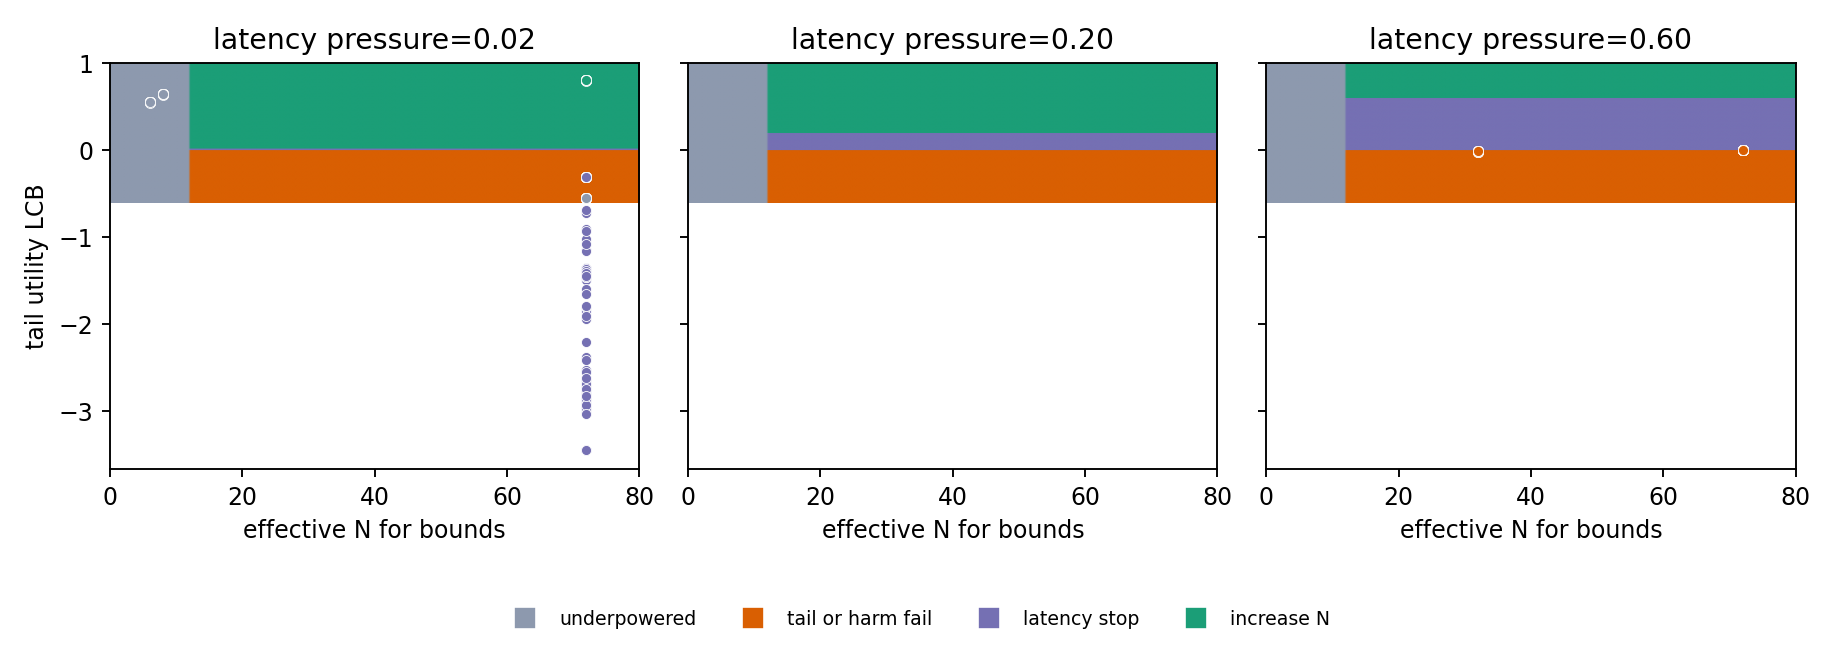
\includegraphics[width=\linewidth]{figures/audit_then_sample_decision_regions.png}
\end{minipage}
\caption{Selection is useful only under the right tail conditions. Left: scorer comparison exposes aligned, calibrated, and misaligned upper-tail behavior. Right: \ats{} admits high $N$ only in certified regions and otherwise emits abstention, repair, diversity, latency, or block actions.}
\label{fig:controller}
\end{figure}

\section{Experiments}

We evaluate six evidence views, each with claim-audited artifacts. Controlled diffusion-like samplers isolate the mechanisms. Learned diffusion-policy-lite models train small state-conditioned and $32{\times}32$ image-conditioned denoisers over action horizons. The main learned diffusion tier trains true epsilon-prediction action DDPM/DDIM samplers, including fast DDIM, stochastic DDPM, one-step consistency-style, and clean-target ablations. The PushT tier uses \texttt{gym\_pusht/PushT-v0} with low-dimensional observations, heuristic demonstrations for CPU-feasible training, sampled action trajectories, and actual simulator rollout utility. The FetchPush tier uses Gymnasium Robotics \citep{towers2024gymnasium} with MuJoCo \citep{todorov2012mujoco} to test the same finite-pool law in a second standard manipulation simulator. A final sequential stress suite alternates aligned, weak-tail, hidden-obstacle, duplicate-artifact, diversity-collapse, latency-spike, calibration-drift, missing-utility, and recovery regimes. The simulator tiers are evidence for the inference-time law, not real-robot or full visual-policy validation.

\begin{table}[t]
\caption{Audited full-run evidence. Gains are high-minus-low selected utility unless noted. The trajectory-search claim is conditional: aligned oracle or calibrated tails can help, while misaligned tails can hurt.}
\label{tab:main-evidence}
\centering
\footnotesize
\begin{tabular}{@{}p{0.16\linewidth}p{0.31\linewidth}p{0.31\linewidth}p{0.11\linewidth}@{}}
\toprule
Tier & Positive evidence & Negative/control evidence & Units \\
\midrule
Controlled sampler & aligned gain $0.601$, \ci{} low $0.550$ & misaligned change $-0.302$, \ci{} high $-0.248$; low-diversity gain $\approx 0$ & 16 seed/state units \\
Controller & 16 admissions; min utility/tail/latency \lcb{}s $0.833/0.802/0.827$ & false-admit rate $0.0$; 112 \texttt{block\_high\_N} actions & 256 rows \\
Deployment stress & static \ats{} exceeds fixed high-$N$ by $\AtsDeployStressStaticVsHigh$ overall; harmful rows $+\AtsDeployStressStaticVsHighHarm$ & fixed high-$N$ harmful in $\AtsDeployStressFixedHighHarmRate$ of rows; aligned/recovery cost $\AtsDeployStressStaticAlignedCost$ & \AtsDeployStressRows{} rows \\
Learned-lite & state gains $0.114$--$0.167$; image gains $0.150$--$0.154$ & supporting tier only; not used for broad visual-policy wording & 3 training seeds \\
True action diffusion & DDIM oracle gain $0.370$, \ci{} low $0.326$; DDPM oracle gain $0.381$, \ci{} low $0.336$ & anti-correlated change $-0.406$, \ci{} high $-0.371$ & 12 seed/state units \\
PushT simulator & utility gain $0.121$, \ci{} low $0.0576$; coverage gain $0.103$, \ci{} low $0.0381$ & harmful reranking $-0.048$, \ci{} high $-0.031$; success gain $0.0$ & 12 paired units \\
FetchPush simulator & utility gain $\AtsFetchBenchmarkAlignedGain$, \ci{} low $\AtsFetchBenchmarkAlignedCILow$; oracle gap $\AtsFetchBenchmarkOracleGap$ & anti-oracle change $\AtsFetchBenchmarkAntiOracleChange$, \ci{} high $\AtsFetchBenchmarkAntiOracleCIHigh$; low-diversity gain $\approx 0$ & \AtsFetchBenchmarkUnits{} paired units \\
\bottomrule
\end{tabular}
\end{table}

\paragraph{Mechanism tests.}
The controlled sampler confirms the finite law. Selected score rises with $N$ even when real utility falls under a misaligned tail; aligned high-diversity selection improves utility; collapsed or low-diversity pools saturate. The latency sweep shows that raw utility is not the only objective: with $U-\lambda C(N,K)$, the best audited budget is $N=32,K=2$, using $6.25\%$ of the largest tested $N{\times}K$ budget and improving the latency-adjusted objective over the high-budget corner by $3.31$ (\ci{} low $3.23$).

\paragraph{Controller audit.}
The controller audit includes aligned pools, anti-correlated scorers, shuffled scorers, adversarial-tail and tail-misaligned scorers, duplicated high-score artifacts, correlated candidate pools, hidden OOD dynamics, missing utility, latency spikes, underpowered audits, adaptive stopping, successful calibration, failed repair, and calibration drift. In the full run, \ats{} has 256 decision rows, admits high $N$ in 16 rows, abstains or chooses another action in 240 rows, has zero false admits in harmful negative controls, and records lower-bound coverage $1.0$. Calibration is intentionally asymmetric: 19 held-out repair rows pass and 45 rows fail or remain negative controls.

\paragraph{Sequential deployment stress.}
We then run \AtsDeployStressRows{} online-style decisions across \AtsDeployStressRegimes{} regimes with fixed low-$N$, fixed high-$N$, oracle high-$N$, static \ats{}, and adaptive \ats{} policies. Fixed high-$N$ is latency-adjusted harmful in \AtsDeployStressFixedHighHarmRate{} of decisions and loses to fixed low-$N$ on harmful rows by \AtsDeployStressFixedHighVsLowHarm{} (\ci{} high \AtsDeployStressFixedHighVsLowHarmCIHigh). Static \ats{} has zero false admits and improves over fixed high-$N$ by \AtsDeployStressStaticVsHigh{} overall (\ci{} low \AtsDeployStressStaticVsHighCILow), by \AtsDeployStressStaticVsHighHarm{} on harmful rows (\ci{} low \AtsDeployStressStaticVsHighHarmCILow), and by \AtsDeployStressStaticVsHighNegative{} on negative regimes (\ci{} low \AtsDeployStressStaticVsHighNegativeCILow). The stress test also exposes a cost: in aligned/recovery regimes, conservative blocking trails fixed high-$N$ by \AtsDeployStressStaticAlignedCost{} (\ci{} high \AtsDeployStressStaticAlignedCostCIHigh). We therefore claim conservative risk control, not free utility.

\begin{figure}[t]
\centering
\begin{minipage}{0.49\linewidth}
\centering
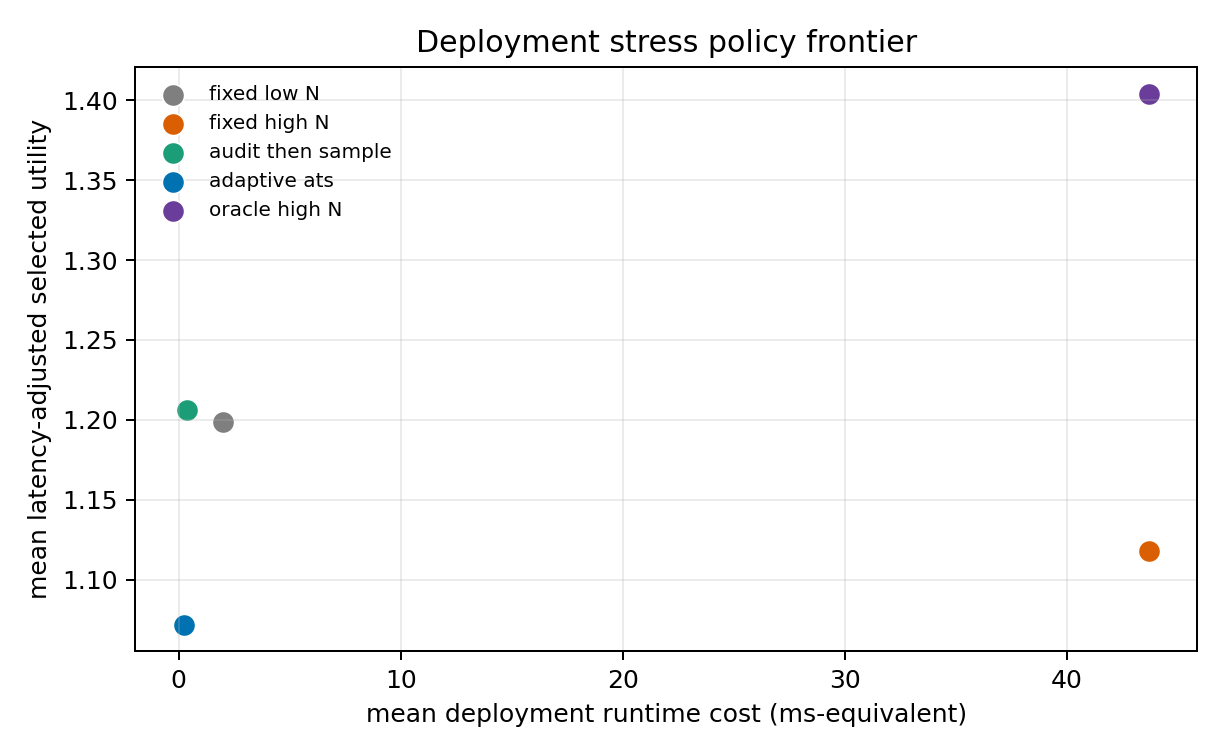
\includegraphics[width=\linewidth]{figures/deployment_stress_frontier.png}
\end{minipage}
\hfill
\begin{minipage}{0.49\linewidth}
\centering
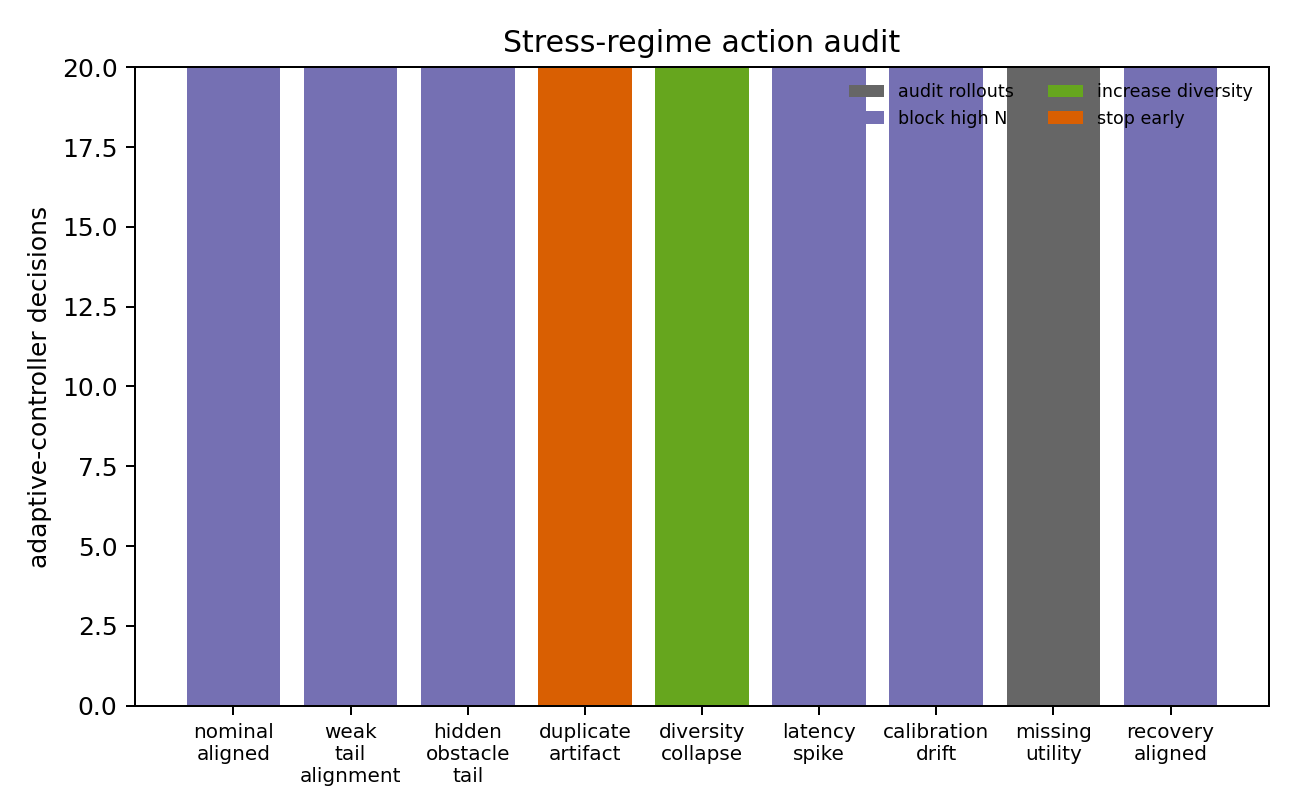
\includegraphics[width=\linewidth]{figures/deployment_stress_actions.png}
\end{minipage}
\caption{Sequential deployment stress. Static \ats{} protects harmful rows relative to fixed high-$N$, while the action audit shows the controller's conservative tendency to block, stop, diversify, or request utility audits under shift.}
\label{fig:deployment-stress}
\end{figure}

\paragraph{Diffusion-policy tiers.}
Learned-lite results support the diagnostic pipeline on learned state and small-image denoisers, but they are not used alone for global diffusion-policy wording. The true action diffusion tier is the main learned evidence: both DDIM and stochastic DDPM oracle reranking have positive lower bounds, while anti-correlated scoring is harmful. Runtime is measured directly, with 540 true-diffusion rows spanning $0.18$ to $13.42$ ms per candidate. PushT supplies simulator rollout evidence: aligned oracle reranking improves utility and coverage, low-diversity gains are small, and a high-temperature misaligned scorer is harmful. FetchPush adds \AtsFetchBenchmarkCandidateRollouts{} MuJoCo rollouts over \AtsFetchBenchmarkUnits{} paired seed/episode units; aligned oracle reranking has positive lower-bound utility gain, low-diversity gains are nearly zero, and anti-oracle tail selection is harmful. PushT runtime spans $104.78$ to $373.44$ ms per candidate; FetchPush spans $\AtsFetchBenchmarkRuntimeMin$ to $\AtsFetchBenchmarkRuntimeMax$ ms per candidate.

\begin{figure}[t]
\centering
\begin{minipage}{0.49\linewidth}
\centering
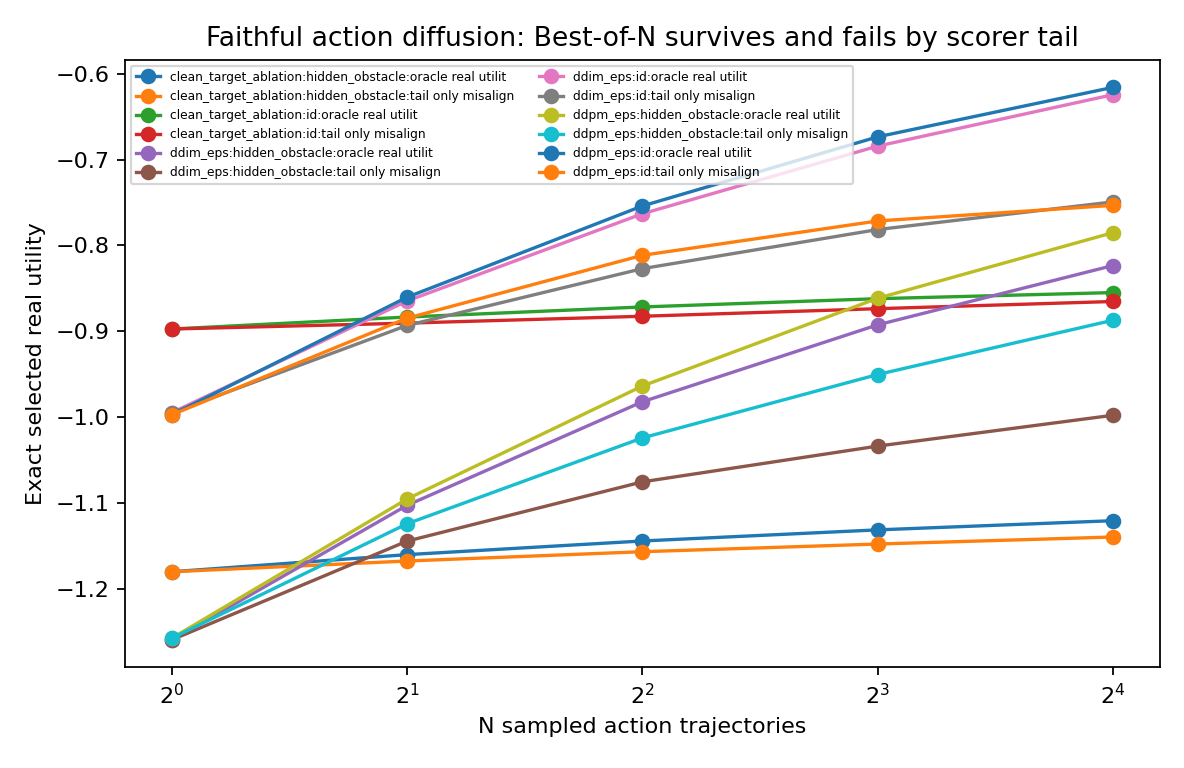
\includegraphics[width=\linewidth]{figures/true_diffusion_survival.png}
\end{minipage}
\hfill
\begin{minipage}{0.49\linewidth}
\centering
\includegraphics[width=\linewidth]{figures/pusht_max_selection.png}
\end{minipage}
\caption{The conditional law survives beyond controlled samplers. Left: true epsilon-prediction action DDPM/DDIM sampling shows aligned oracle gains and harmful negative controls. Right: PushT simulator rollouts show aligned utility and coverage gains, low-diversity saturation, and misaligned-scorer failure.}
\label{fig:diffusion-pusht}
\end{figure}

\section{Related Work}

Diffusion models turn iterative denoising into a flexible generative mechanism \citep{sohl2015deep,ho2020ddpm,song2020ddim}; Diffusion Policy applies this idea to visuomotor action sequence generation and highlights multimodal action distributions \citep{chi2023diffusionpolicy}. Test-time reranking and verifier-based selection are common in sequence generation and decision problems \citep{cobbe2021training,yao2023tree}, but selected-score maximization is only useful when the score tail reflects the target utility. In robotics and imitation learning, value critics, behavior-cloning scores, implicit policies, and offline trajectory models provide possible rerankers or action generators \citep{florence2022implicit,janner2022diffuser,mandlekar2021robomimic}. Standard simulator interfaces such as Gymnasium Robotics and MuJoCo make it possible to audit those inference-time effects under recognized manipulation dynamics \citep{towers2024gymnasium,todorov2012mujoco}. Our focus is narrower: a finite audit of when increasing sampled diffusion trajectories is certified, harmful, saturated, or latency-dominated.

\section{Audit Discipline and Limitations}

All promoted claims must pass the claim audit. The full-run audit reports \texttt{all\_strong=true}, 20 supported claims, no partial or unsupported claims, no full-run low-power warning, true-DDPM, PushT, and FetchPush gates supported, negative controls present, runtime evidence present, and no real-robot or full visual-policy overclaim. Main-text numbers in Tables~\ref{tab:main-evidence} and \ref{tab:artifact-map-short} are backed by the appendix artifact map and anonymous supplementary material.

The evidence is CPU simulation evidence. The controlled sampler is hand-designed. The learned-lite tier is intentionally small. The image-conditioned path uses $32{\times}32$ toy renderings and a tiny CNN. The true action diffusion tier uses faithful epsilon-prediction DDPM/DDIM action sampling, but on a small toy manipulation dataset. PushT and FetchPush are simulator benchmark paths with low-dimensional observations and heuristic demonstrations. We do not claim real-robot validation, universal Diffusion Policy improvement, hardware safety certification, or full visual imitation-learning validation.

\begin{table}[t]
\caption{Main artifact pointers. Repo-relative paths are kept in the appendix and anonymous supplement; public personal links are not used.}
\label{tab:artifact-map-short}
\centering
\small
\begin{tabular}{@{}p{0.22\linewidth}p{0.31\linewidth}p{0.28\linewidth}@{}}
\toprule
Claim family & Primary tables & Primary figures \\
\midrule
Finite law and diversity & \path{controlled_sampler_effect_cis.csv}; \path{controlled_sampler_diversity.csv} & \path{controlled_sampler_curves.png} \\
Controller and repair & \path{audit_then_sample_decisions.csv}; \path{audit_then_sample_calibration.csv} & \path{audit_then_sample_decision_regions.png} \\
Deployment stress & \path{deployment_stress_decisions.csv}; \path{deployment_stress_policy_effect_cis.csv} & \path{deployment_stress_frontier.png}; \path{deployment_stress_actions.png} \\
Runtime & \path{nk_budget_latency_effect_ci.csv}; \path{true_diffusion_runtime.csv}; \path{pusht_runtime.csv}; \path{fetch_robotics_runtime.csv} & \path{nk_budget_phase_diagram.png}; \path{true_diffusion_runtime.png} \\
True DDPM/DDIM and benchmarks & \path{true_diffusion_effect_cis.csv}; \path{pusht_rollout_metric_effect_cis.csv}; \path{fetch_robotics_effect_cis.csv} & \path{true_diffusion_survival.png}; \path{pusht_max_selection.png}; \path{fetch_robotics_selection.png} \\
\bottomrule
\end{tabular}
\end{table}

\section{Conclusion}

High-$N$ diffusion-policy inference is conditionally useful, not universally beneficial. More samples help when the candidate pool is diverse, the scorer's upper tail selects genuinely high-utility trajectories, and latency cost is dominated by the utility gain. More samples saturate when diversity collapses and can hurt when the scorer's tail is misaligned. \ats{} turns this into a conservative deployment-facing rule: certify high $N$ with lower-bound audit evidence, otherwise abstain, audit, repair, reduce compute, increase diversity, or block high-$N$ selection.

\section*{Reproducibility Statement}
The anonymous supplementary material contains source code, result CSV/JSON artifacts, figure-generation outputs, seeds, hyperparameters, and exact reproduction commands. The theorem implementation is tested in \texttt{tests/test\_theory.py}; claim promotion is gated by \texttt{scripts/run\_claim\_audit.sh}; and the paper build is checked by \texttt{scripts/build\_iclr\_paper.py}. Appendix~\ref{app:repro} maps each main claim to tracked artifacts.

\section*{Ethics and Impact Statement}
This work studies inference-time sampling decisions in CPU simulation. It does not use human subjects, private data, real-robot deployment, or safety-critical hardware trials. The main risk is over-interpreting simulated audit evidence as a hardware safety guarantee; the paper explicitly blocks that interpretation and requires fresh task-specific audits before using high-$N$ sampling in new settings.

\section*{LLM Usage Statement}
Large language models were used as general-purpose assistance for drafting, editing, and packaging. The authors are responsible for all claims, citations, experiments, and final text. No LLM-generated empirical results are reported.

\phantomsection\label{maintextend}
\bibliography{references}
\bibliographystyle{iclr2026_conference}

\appendix
\section{Proof Details}
\label{app:proof}

For a fixed observation, consider a finite candidate pool of size $M$ sorted by nondecreasing score. Let $g$ index one score-tie group with ranks $a_g,\ldots,b_g$. The event that the maximum sampled score falls in group $g$ is the event that all $N$ draws have rank at most $b_g$ and at least one draw has rank at least $a_g$. With replacement, this probability is
\[
\left(\frac{b_g}{M}\right)^N -
\left(\frac{a_g-1}{M}\right)^N.
\]
Conditional on this event and uniform tie-breaking inside the group, the selected utility contribution is the tied-group mean $\bar U_g$. Summing over disjoint tie groups gives Equation~\ref{eq:finite-law}. Replacing $\bar U_g$ with the tied-group mean score gives the selected-score expression. Selected score is nondecreasing in $N$ because it is the expectation of a sample maximum. Selected utility has no such monotonicity unless high-score tail groups have nondecreasing utility contributions.

\section{Controller Gate Details}
\label{app:controller}

\ats{} uses one-sided lower-bound gates for admission. The full run uses candidate-pool diagnostics from \texttt{results/tables/audit\_then\_sample\_decisions.csv} and repair diagnostics from \texttt{results/tables/audit\_then\_sample\_calibration.csv}. An \texttt{increase\_N} decision is admitted only when the diversity gate passes, the high-minus-low utility lower bound is positive, the top-score-tail utility lower bound is positive, the latency-adjusted gain lower bound is positive, and the high-score-tail harm upper bound does not indicate plausible harm. Missing utility routes to \texttt{audit\_rollouts} or \texttt{calibrate\_scorer}; collapsed diversity routes to \texttt{increase\_diversity}; anti-alignment routes to \texttt{block\_high\_N}; and finite latency optima route to \texttt{stop\_early} or \texttt{reduce\_K}.

\begin{table}[H]
\caption{Controller audit summary from the full run.}
\label{tab:controller-full}
\centering
\small
\begin{tabular}{lr}
\toprule
Quantity & Value \\
\midrule
Decision rows & 256 \\
\texttt{increase\_N} admissions & 16 \\
Abstentions or non-\texttt{increase\_N} actions & 240 \\
\texttt{block\_high\_N} actions & 112 \\
False admits in harmful negative controls & 0 \\
Empirical-Bernstein lower-bound coverage & 1.0 \\
Adaptive stopping savings mean & 0.667 \\
Calibration success / failure rows & 19 / 45 \\
\bottomrule
\end{tabular}
\end{table}

\section{Experiment Configuration}
\label{app:configs}

\begin{table}[H]
\caption{Primary experimental configurations.}
\label{tab:configs}
\centering
\small
\begin{tabular}{@{}p{0.22\linewidth}p{0.65\linewidth}@{}}
\toprule
Tier & Configuration \\
\midrule
Controlled sampler & Sixteen seed/state units; high-diversity aligned and misaligned regimes; low-diversity and collapsed regimes; $N$ grid up to 64; exact finite-pool curves and paired confidence intervals. \\
\ats{} audit & Aligned, anti-correlated, shuffled, adversarial-tail, tail-misaligned, duplicated-artifact, correlated-pool, hidden-OOD, missing-utility, latency-spike, underpowered, adaptive-stopping, repair-success, repair-failure, and calibration-drift regimes. \\
Deployment stress & Four seeds, five episodes per regime, nine sequential regimes, 96 candidates, $K\in\{2,8,16\}$, fixed low-$N$, fixed high-$N$, oracle high-$N$, static \ats{}, and adaptive \ats{} policy comparisons. \\
Learned-lite & Three training seeds; state-conditioned MLP denoiser and $32{\times}32$ image-conditioned tiny-CNN denoiser; action horizons; ID and OOD regimes; receding-horizon evaluation. \\
True action diffusion & Four training seeds and three evaluation states, giving 12 paired seed/state units for key confidence rows; epsilon-prediction DDPM objective; DDIM, stochastic DDPM, one-step consistency-style, and clean-target ablation samplers. \\
PushT simulator & Four training seeds and three evaluation episodes, giving 12 paired seed/episode units; horizon 20; 16 candidates; $K\in\{1,8,16\}$; aligned, low-diversity, and high-temperature misaligned regimes; actual simulator rollout utility and coverage metrics. \\
FetchPush simulator & Four training seeds and three evaluation episodes, giving 12 paired seed/episode units; horizon 14; 8 candidates; $K\in\{1,8\}$; Gymnasium Robotics FetchPush-v4 MuJoCo rollouts; aligned, low-diversity, and high-temperature anti-tail regimes. \\
\bottomrule
\end{tabular}
\end{table}

\section{Artifact Map and Claim Ledger}
\label{app:repro}

The package uses repo-relative paths only. The anonymous supplement contains the same source and result artifacts without author-identifying links.

\begin{table}[H]
\caption{Artifact map for the main evidence stack.}
\label{tab:artifact-map-full}
\centering
\small
\begin{tabular}{@{}p{0.18\linewidth}p{0.35\linewidth}p{0.30\linewidth}@{}}
\toprule
Family & Tables and summaries & Figures \\
\midrule
Claim audit & \path{claims_status.*}; \path{ideal_metrics_status.*} & none \\
Controlled sampler & \path{controlled_sampler_summary.json}; curves, diversity, and effect-CI CSVs & \path{controlled_sampler_curves.png} \\
Controller & \path{audit_then_sample_summary.json}; decision and calibration CSVs & \path{audit_then_sample_decision_regions.png} \\
Deployment stress & \path{deployment_stress_summary.json}; decision, policy, and effect-CI CSVs & \path{deployment_stress_frontier.png}; \path{deployment_stress_actions.png} \\
Scorers and repair & \path{scorer_comparison_summary.json}; curves, effect-CI, and repair-map CSVs & \path{scorer_comparison.png} \\
Latency & \path{nk_budget_summary.json}; phase, latency-CI, and runtime CSVs & \path{nk_budget_phase_diagram.png}; \path{true_diffusion_runtime.png} \\
Learned-lite & \path{learned_policy_lite_summary.json}; training, effect-CI, and receding-horizon CSVs & \path{learned_policy_lite_ood.png}; \path{toy_image_observations.png} \\
True DDPM/DDIM & \path{true_diffusion_summary.json}; curves, effect-CI, runtime, and sampler-comparison CSVs & \path{true_diffusion_survival.png}; \path{true_diffusion_sampler_comparison.png} \\
PushT & \path{pusht_summary.json}; curves, rollout, rollout-metric, and runtime CSVs & \path{pusht_max_selection.png} \\
FetchPush & \path{fetch_robotics_summary.json}; curves, rollout, rollout-metric, and runtime CSVs & \path{fetch_robotics_selection.png} \\
\bottomrule
\end{tabular}
\end{table}

\begin{table}[H]
\caption{Claim audit ledger. All promoted claims are supported in the full run.}
\label{tab:claim-ledger}
\centering
\small
\begin{tabular}{@{}p{0.07\linewidth}p{0.70\linewidth}p{0.10\linewidth}@{}}
\toprule
ID & Claim family & Status \\
\midrule
1 & Finite tie-aware maximum-score selection law is implemented and tested. & Supported \\
2--4 & High $N$ can help aligned selection, hurt or saturate under misalignment, and saturate under low diversity. & Supported \\
5--7 & $N$ versus $K$ tradeoff, latency-adjusted finite optima, and at least one calibrated repair regime. & Supported \\
8 & \ats{} chooses among increase, stop, repair, diversity, reduce-$K$, audit, and block actions with no harmful false admits. & Supported \\
9 & Sequential deployment stress has zero false admits and quantifies conservative opportunity cost. & Supported \\
10--12 & Differentiation from adjacent projects and artifact-backed claim discipline. & Supported \\
13 & Learned diffusion-policy-lite validity checklist and multi-seed state/image evaluation. & Supported \\
14 & True epsilon-prediction action DDPM/DDIM effects survive with one-step and clean-target ablations. & Supported \\
15--16 & PushT simulator reranking law, rollout coverage, and success curves over actual simulator rollouts. & Supported \\
17 & FetchPush-v4 Gymnasium Robotics/MuJoCo rollout bridge over 12 paired units. & Supported \\
18--20 & Runtime-backed recommendations, global wording gated on true-DDPM plus PushT plus FetchPush, and reviewer-skepticism checklist. & Supported \\
\bottomrule
\end{tabular}
\end{table}

\section{Reviewer Concern Matrix}
\label{app:concerns}

\begin{table}[H]
\caption{Pre-registered concern-to-evidence mapping.}
\label{tab:concerns}
\centering
\small
\begin{tabular}{@{}p{0.24\linewidth}p{0.37\linewidth}p{0.25\linewidth}@{}}
\toprule
Concern & Paper answer & Direct artifact \\
\midrule
High $N$ helps everywhere. & Misaligned controlled, true-diffusion, PushT, and FetchPush anti-tail controls expose harmful high-$N$ selection. & \path{results/claims_status.md}, Claims 3, 14, 15, 17 \\
The controller admits unsafe high $N$. & Harmful negative controls have zero false admits; admitted rows have positive utility, tail, and latency lower bounds. & \path{audit_then_sample_summary.json}; \path{audit_then_sample_decisions.csv} \\
The controller is too conservative. & Deployment stress reports both protection and cost: zero false admits and positive harmful-row gains, but aligned/recovery rows trail fixed high-$N$. & \path{deployment_stress_policy_effect_cis.csv}, Claim 9 \\
This is only a toy sampler. & Global wording requires true-DDPM, PushT, and FetchPush rollout-metric gates; learned-lite and controlled tiers are supporting context. & \path{ideal_metrics_status.json}, Claims 13--20 \\
Runtime is ignored. & Budget sweeps and measured true-diffusion, PushT, and FetchPush runtimes are audited. & \path{nk_budget_latency_effect_ci.csv}; runtime CSVs \\
Repair always works. & Calibration has both success and failure rows; repair is used only under held-out lower-bound gates. & \path{audit_then_sample_calibration.csv} \\
Robot validity is overstated. & Scope excludes real robots, hardware safety, production visual policies, and full visual benchmark validation. & \path{paper/limitations.md}; \path{ideal_metrics_status.json} \\
\bottomrule
\end{tabular}
\end{table}

\section{Reproduction Commands}
\label{app:commands}

From the repository root:
\begin{verbatim}
python scripts/build_iclr_paper.py
bash scripts/run_claim_audit.sh
python scripts/run_with_src.py experiments/deployment_stress.py
python -m pytest -q
rg -n "F(?:INAL RERUN)" paper docs README.md
rg -n "T(?:ODO)|placehold(?:er)" paper docs README.md
rg -n "almost\s+100|100[%]" paper docs README.md
rg -n "validated on real robot[s]" paper docs README.md
rg -n "trajectory search always help[s]" paper docs README.md
\end{verbatim}
The paper PDF is written to \texttt{paper/iclr/main.pdf}, copied to \texttt{paper/iclr/final/best of n diffusion policy-v4.pdf}, and mirrored to \texttt{paper/final/best of n diffusion policy-v4.pdf}. The build wrapper compiles with the official ICLR 2026 style proxy and fails if the page label immediately before references exceeds nine pages.

\section{LLM Usage Details}
\label{app:llm}

LLM tools were used for drafting assistance, wording compression, checklist generation, and packaging mechanics. They were not used to fabricate empirical outputs. All numerical claims are taken from tracked CSV/JSON artifacts and must pass the claim-audit script before promotion.


\end{document}
